\documentclass{article}
\usepackage{tikz}

\begin{document}

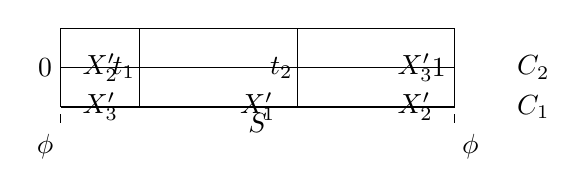
\begin{tikzpicture}[scale=1]
    % Draw the horizontal lines
    \draw (0,0) -- (5,0);
    \draw (0,1) -- (5,1);
    
    % Draw the vertical lines
    \draw (0,0) -- (0,1);
    \draw (1,0) -- (1,1);
    \draw (3,0) -- (3,1);
    \draw (5,0) -- (5,1);
    
    % Label the vertical lines
    \node at (-0.2, 0.5) {$0$};
    \node at (1-0.2, 0.5) {$t_1$};
    \node at (3-0.2, 0.5) {$t_2$};
    \node at (5-0.2, 0.5) {$1$};
    
    % Draw the horizontal line separating the two regions
    \draw (0,0.5) -- (5,0.5);
    
    % Label the horizontal line
    \node at (2.5, -0.2) {$S$};
    
    % Label the regions
    \node at (0.5, 0.5) {$X'_2$};
    \node at (4.5, 0.5) {$X'_3$};
    \node at (0.5, 0) {$X'_3$};
    \node at (2.5, 0) {$X'_1$};
    \node at (4.5, 0) {$X'_2$};
    
    % Label the vertical distances
    \node at (6, 0.5) {$C_2$};
    \node at (6, 0) {$C_1$};
    
    % Dashed lines indicating the boundary of the region
    \draw[dashed] (0,-0.2) -- (0,0.2);
    \draw[dashed] (5,-0.2) -- (5,0.2);
    
    % Labels for the dashed lines
    \node at (-0.2, -0.5) {$\phi$};
    \node at (5.2, -0.5) {$\phi$};
\end{tikzpicture}

\end{document}